\section{Problem (5)}
	You throw a ball toward a wall at speed $25 \ m/s$ and at angle $\theta_{0} = 38^{o}$ above the horizontal. The wall is distance $d = 17 \ m$ from the release point of the ball.

	\begin{figure}[H]
		\begin{center}
			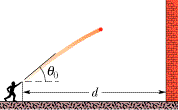
\includegraphics[scale=1]{hw4_problem5}
			\caption{Illustration of Problem 5}
			\label{fig:hw4_problem5}
		\end{center}
	\end{figure}

	\subsection{Question (a)}
		How far above the release point does the ball hit the wall?

		\textbf{R:} \newline
		\begin{align}
			v_{0_{x}} = \ &v \cos 38^{o}& \notag \\
			= \ &(25 \ m/s)(0.7880) = 19.7000 \ m/s& \notag \\
			x = \ &x_{0} + v_{0_{x}}t + \frac{1}{2}a_{x}t^{2}& \notag \\
			17 \ m = \ &(19.7 \ m/s)t& \notag \\
			t = \ &\frac{17 \ m}{19.7 \ m/s} = 0.8629 \ s& \notag \\
			v_{0_{y}} = \ &v \sin 38^{o}& \notag \\
			= \ &(25 \ m/s)(0.6157) = 15.3925 \ m/s& \notag \\
			y = \ &y_{0} + v_{0_{y}}t + \frac{1}{2}a_{y}t^{2}& \notag \\
			= \ &(15.3925 \ m/s)(0.8629 \ s) + \left(-4.9 \ m/s^{2} \right)(0.8629 \ s)^{2}& \notag \\
			= \ &(13.2821 \ m) - (3.6485 \ m) = 9.6336 \ m&
		\end{align}

	\subsection{Question (b)}
		What is the horizontal component of its velocity as it hits the wall?

		\textbf{R:} \newline
		\begin{align}
			v_{x} = \ &v_{0_{x}} + a_{x}t = v_{0_{x}}& \notag \\
			= \ &19.7000 \ m/s&
		\end{align}

	\subsection{Question (c)}
		What is the vertical component of its velocity as it hits the wall?

		\textbf{R:} \newline
		\begin{align}
			v_{y} = \ &v_{0_{y}} + a_{y}t& \notag \\
			= \ &(15.3925 \ m/s) + \left( -9.8 \ m/s^{2} \right)(0.8629 \ s)& \notag \\
			= \ &(15.3925 \ m/s) - (8.4564 \ m/s) = 6.9361 \ m/s&
		\end{align}
